\documentclass[a4paper,11pt,romanian]{article}
\usepackage[colorlinks,allcolors=black,unicode]{hyperref}
\usepackage{graphicx}
\usepackage{graphics}
\usepackage{combelow}
\usepackage{hyperref}
\usepackage[utf8x]{inputenc}
\usepackage{cite}

\author{David Harabagiu \& Diana Bejan\\30239 \& 302310\\Prof. Coordonator Dan Butiri}
\title{\uppercase{\textbf{Departamentul de calculatoare} \vspace{20.0pt} \\ utilizarea portului vga al pl\u{a}cii basys 3 pentru afi\cb{s}area unor imagini}}
\renewcommand{\refname}{Referin\cb{t}e}
\renewcommand{\figurename}{Fig.}
\renewcommand{\contentsname}{Con\cb{t}inut}
\renewcommand{\tablename}{Tabel}

\begin{document}
\begin{figure}
  \begin{center}
   
\includegraphics[scale=0.1]{utcn.png}
   \label{fig:utcnlogo}
  \end{center}
 \end{figure}
\maketitle
\newpage
\tableofcontents
\newpage

\section{Rezumat}

Acest document prezin\u{a} o scurt\u{a} sintez\u{a} cu privire la realizarea unui circuit numeric pe o plac\u{a} de dezvoltare Basys 3 FPGA, capabil s\u{a} utilizeze portul VGA al acesteia pentru afi\cb{s}area unor imagini pe un display.
Problema principal\u{a} este cea a conducerii semnalelor portului VGA, astfel \^{i}nc\^{a}t acestea s\u{a} fie sincronizate corect.
Alte obiective cuprind manipularea culorilor cu ajutorul unor filtre de imagini ce pot fi schimbate de c\u{a}tre utilizator cu ajutorul unor comutatoare \cb{s}i crearea unei aplica\cb{t}ii interactive care s\u{a} determine ie\cb{s}irea \^{i}n func\cb{t}ie de stimulii utilizatorului.
Pentru dezvoltare, a fost ales limbajul VHDL \cb{s}i mediul de dezvoltare Xilinx Vivado 2017.4. Un alt utilitar folosit, de origine proprie, este o aplica\cb{t}ie ce genereaz\u{a}, pe baza unei imagini un modul VHDL ce reprezint\u{a} un look-up table cu informa\cb{t}iile de culoare ale imaginii.
Pentru versionarea codului surs\u{a} a fost utilizat Git.
Rezultatul este o aplica\cb{t}ie versatil\u{a} ce are un poten\cb{t}ial ridicat de dezvoltare ulterioar\u{a} \^{i}n lumea noastr\u{a} de consumatori media.

\newpage

\section{Introducere}
Video Graphics Array (VGA) este hardware-ul de afi\cb{s}are ce a fost introdus \^{i}mpreun\u{a} cu seria de calculatoare IBM PS/2 \^{i}n anul 1987, succesor al CGA \cb{s}i EGA introduse \^{i}n calculatoarele personale IBM dezvoltate anterior. VGA a fost ultimul standard grafic IBM c\u{a}ruia i s-au conformat majoritatea produc\u{a}torilor de calculatoare, f\u{a}c\^{a}ndu-l standardul fundamental ce tot hardware-ul grafic post-1990 ar fi trebuit s\u{a} \^{i}l implementeze. Ast\u{a}zi, interfa\cb{t}a VGA analog este utilizat\u{a} pentru video la calitate \^{i}nalt\u{a}, inclusiv rezolu\cb{t}ii 1080p sau mai mari. ~\cite{wiki:vga}

VGA este considerat mai mult un "Array" dec\^{a}t un "adaptor" deoarece a fost implementat de la \^{i}nceput ca un singur cip ce a \^{i}nlocuit at\^{a}t  generatorul de adrese video Motorola 6845 c\^{a}t \cb{s}i alte zeci de circuite logice discrete ce acopereau complet pl\u{a}cile ISA ale MDA, CGA \cb{s}i EGA. Implementarea pe un singur cip a permis ca VGA s\u{a} fie amplasat direct pe placa de baz\u{a} a unui PC cu dificultate minim\u{a}, deoarece erau necesare doar o memorie video, oscilatoare \cb{s}i un RAMDAC extern. A\cb{s}adar, primele modele IBM PS/2 erau echipate cu VGA pe placa de baz\u{a}, \^{i}n contrast cu modele mai vechi ce necesitau un adapotor de afi\cb{s}are instalat \^{i}ntr-un slot pentru a conecta un monitor. VGA folose\cb{s}te conectorul DE-HD15. ~\cite{wiki:vga}

Obiectivul acestui proiect este de a demonstra func\cb{t}ionalit\u{a}\cb{t}ile VGA, prin implementarea unui controller pe o plac\u{a} FPGA (Field-programmable gate array) \cb{s}i utilizarea port-ului pl\u{a}cii pentru a afi\cb{s}a imagini pe un monitor. S-au implementat aplica\cb{t}ii cum ar fi afi\cb{s}area fotografiilor, aplicarea filtrelor de imagini (negativ, controlul contrastului, grayscale, dezactivarea individual\u{a} a canalelor Red, Green, Blue), precum \cb{s}i o aplica\cb{t}ie interactiv\u{a} - o implementare a jocului Snake.

\^{I}n solu\cb{t}ia propus\u{a} am separat partea de controller VGA de aplica\cb{t}iile asociate men\cb{t}ionate anterior. Controller-ul folose\cb{s}te 2 num\u{a}r\u{a}toare pentru a genera semnalele de sincronizare orizontal\u{a} \cb{s}i vertical\u{a}, precum \cb{s}i semnalele de adresare a memoriei video.  Implementarea aleas\u{a} utilizeaz\u{a} modul video VGA 640x480@60Hz. Datorit\u{a} anumitor limit\u{a}ri hardware (memoria disponibil\u{a} pe placa de dezvoltare FPGA), fotografiile stocate au o dimensiune de 160x120, iar apoi sunt redimensionate de c\u{a}tre hardware, semnalele digitale de adresare fiind \^{i}mp\u{a}r\cb{t}ite cu 4 \^{i}naintea select\u{a}rii pixelului din fotografie. Pentru a controla aplica\cb{t}ia interactiv\u{a}, este utilizat\u{a} comunicarea cu o tastatur\u{a} PS/2 prin portul disponibil pe placa de dezvoltare.

\^{I}n sec\cb{t}iunea "Fundamentare teoretic\u{a}" se prezint\u{a} fundamentele teoretice legate de VGA, portul PS/2 \cb{s}i filtrele de imagini. Sec\cb{t}iunea "Proiectare \cb{s}i implementare" prezint\u{a} detalii tehnice legate de implementarea aleas\u{a}, cum s-a ajuns la aceast\u{a} solu\cb{t}ie, precum \cb{s}i un ghid pentru configurarea \cb{s}i utilizarea aplica\cb{t}iei. \^{I}n sec\cb{t}iunea "Rezultate experimentale" sunt prezentate informa\cb{t}ii relevante \cb{s}i rezultate ale simul\u{a}rii \cb{s}i implement\u{a}rii.

\section{Fundamentare teoretic\u{a}}

\subsection{VGA (Video Graphics Array)}
\small{ 

VGA (Video Graphics Array) se refer\u{a} de obicei la standardele de afi\cb{s}are analog a calculatoarelor, la conectorul DE-15 (cunoscut ca \cb{s}i conectorul VGA) sau la rezolu\cb{t}ia 640x480.

Conectorul DE-15 este un conector cu 15 pini amplasa\cb{t}i in 3 r\^{a}nduri. Numele fiec\u{a}rui pin este specificat \^{i}n Fig.\ref{fig:vgaconnector}.
\begin{figure}
  \begin{center}
   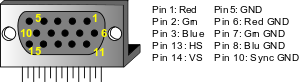
\includegraphics[scale=0.55]{VGA_Connector.png}
   \caption{Conectorul VGA}
   \label{fig:vgaconnector}
  \end{center}
 \end{figure}
 Semnalele Red, Grn, Blue sunt 3 semnale analog ce specific\u{a} culoarea unui punct de pe ecran, pe c\^{a}nd HS \cb{s}i VS ne dau o referin\cb{t}\u{a} pozi\cb{t}ional\u{a} despre unde ar trebui ca punctul s\u{a} fie afi\cb{s}at. 
Display-urile VGA bazate pe CRT folosesc raze de electroni modulate de amplitudine ce se mi\cb{s}c\u{a} pentru a afi\cb{s}a informa\cb{t}ii pe un ecran cu pelicul\u{a} de fosfor. Display-urile LCD folosesc o matrice de comutatoare ce impun un voltaj pe o suprafa\cb{t}\u{a} mic\u{a} de cristal lichid. Chiar dac\u{a} urmatoarea descriere este limitat\u{a} la monitoarele CRT, cele LCD au evoluat pentru a utiliza aceia\cb{s}i timpi de semnal ca \cb{s}i cele CRT. Monitoarele CRT multicolor folosesc 3 raze de electroni (pentru ro\cb{s}u, verde \cb{s}i albastru) pentru a energiza pelicula de fosfor de pe partea interioar\u{a} a ecranului (Fig.\ref{fig:crtmonitor}).
\begin{figure}
  \begin{center}
   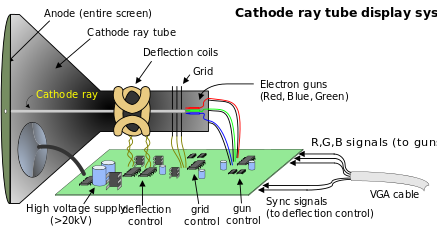
\includegraphics[scale=0.55]{CRT_Monitor.png}
   \caption{Monitor CRT Multicolor}
   \label{fig:crtmonitor}
  \end{center}
 \end{figure}

Informa\cb{t}ia este afi\cb{s}at\u{a} doar atunci c\^{a}nd raza se mi\cb{s}c\u{a} "\^{i}nainte" (de la st\^{a}nga la dreapta \cb{s}i de sus \^{i}n jos), \cb{s}i nu c\^{a}nd raza este resetat\u{a} \^{i}n col\cb{t}ul st\^{a}nga sus a ecranului. Astfel, mult timp poten\cb{t}ial pentru afi\cb{s}are este pierdut \^{i}n perioadele de "blanking", c\^{a}nd raza este resetat\u{a} \cb{s}i stabilizat\u{a} \cb{s}i \^{i}ncepe o nou\u{a} trecere orizontal\u{a} sau vertical\u{a}. Dimensiunea razei, frecven\cb{t}a cu care raza este trasat\u{a} de-a lungul ecranului \cb{s}i frecven\cb{t}a la care raza poate fi modulat\u{a} determin\u{a} rezolu\cb{t}ia.

Display-urile moderne VGA pot acomoda diferite rezolu\cb{t}ii, iar un circuit de control VGA dicteaz\u{a} rezolu\cb{t}ia prin producerea diferitor semnale de timp. Controller-ul trebuie s\u{a} produc\u{a} pulsuri de sincronizare la 3.3V (sau 5V) pentru a seta frecven\cb{t}a cu care curentul se deplaseaz\u{a} prin bobinele de deflec\cb{t}ie, \cb{s}i trebuie s\u{a} se asigure c\u{a} datele video sunt aplicate la timpul potrivit. Display-urile definesc un num\u{a}r de "r\^{a}nduri" ce corespund unui num\u{a}r de treceri orizontale \cb{s}i un num\u{a}r de "coloane" care corespund unei suprafe\cb{t}e pe fiecare r\^{a}nd ce este atribuit\u{a} unui pixel.

Datele video vin de obicei vin de obicei dintr-o memorie video refresh, cu unul sau mai mul\cb{t}i bytes atribui\cb{t}i fiec\u{a}rui pixel. Basys 3 utilizeaz\u{a} 12 bi\cb{t}i pe pixel. Controller-ul trebuie s\u{a} indexeze \^{i}ntr-o memorie video \^{i}n timp ce raza se mi\cb{s}c\u{a} pe ecran, \cb{s}i s\u{a} aplice informa\cb{t}ia despre pixel la timpul precis \^{i}n care raza se mi\cb{s}c\u{a} deasupra acelui pixel.

Un controller VGA trebuie s\u{a} genereze semnalele de timp HS \cb{s}i VS pentru a coordona transmisia de date video pe baza unui semnal de tact "Pixel Clock". Acest semnal de tact define\cb{s}te timpul disponibil pentru a afi\cb{s}a un pixel. Semnalul VS define\cb{s}te rata de "refresh" a ecranului. Num\u{a}rul de linii de afi\cb{s}at define\cb{s}te rata de "retrace" orizontal. ~\cite{misc:digilent}

\begin{figure}
  \begin{center}
   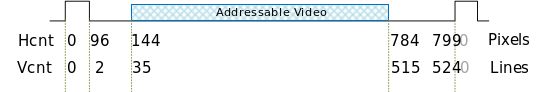
\includegraphics[scale=0.5]{VGA_HSVS.png}
   \caption{Generarea HS \cb{s}i VS pe baza valorilor num\u{a}r\u{a}toarelor}
   \label{fig:hsvsgen}
  \end{center}
 \end{figure}

\subsection{Tastatura PS/2}

\begin{figure}
  \begin{center}
   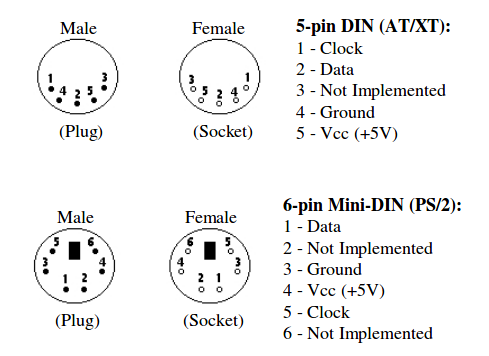
\includegraphics[scale=0.5]{ps2pinout.png}
   \caption{Configura\cb{t}ia pinilor PS/2}
   \label{fig:ps2pinout}
  \end{center}
 \end{figure}
\small{Portul fizic PS/2 poate fi de 2 feluri: cu 5 pini sau cu 6 pini, singura diferen\cb{t}\u{a} fiind aranjarea pinilor. Configura\cb{t}ia pinilor este afi\cb{s}at\u{a} in Fig.\ref{fig:ps2pinout}.
Vcc/Ground asigur\u{a} putere dispozitivului. Liniile Data si Clock sunt am\^{a}ndou\u{a} open collector cu rezisten\cb{t}e pullup la Vcc. O interfa\cb{t}\u{a} open-collector are 2 st\u{a}ri posibile: low \cb{s}i impedan\cb{t}\u{a} \^{i}nalt\u{a}. \^{I}n starea low, un tranzistor trage linia la ground. \^{I}n starea de impedan\cb{t}a \^{i}nalt\u{a}, interfa\cb{t}a se comport\u{a} ca un circuit deschis si nu trage linia nici jos nici sus. O rezisten\cb{t}\u{a}  pullup este conectat\u{a} \^{i}ntre magistral\u{a} si Vcc astfel \^{i}nc\^{a}t magistrala este tras\u{a} sus dac\u{a} niciun dispozitiv de pe magistral\u{a} nu o trage jos.

Mouse-ul si tastatura PS/2 implementeaz\u{a} un protocol serial bidirec\cb{t}ional sincron. Magistrala este "idle" c\^{a}nd am\^{a}ndou\u{a} linii sunt sus. Aceasta este singura stare \^{i}n care dispozitivului \^{i}i este permis s\u{a} transmit\u{a} date. Gazda este singura ce are control deplin asupra magistralei si poate inhiba comunicarea \^{i}n orice moment prin tragerea linei Clock jos. Dispozitivul genereaz\u{a} mereu un semnal de tact.

Toate datele sunt transmise cu c\^{a}te un byte pe rand. Fiecare byte este transmis \^{i}ntr-un cadru con\cb{t}in\^{a}nd 11-12 bi\cb{t}i. Ace\cb{s}ti bi\cb{t}i sunt:
\begin{itemize}
\item 1 bit de start, \^{i}ntotdeauna 0;
\item bi\cb{t}i de date, cel mai pu\cb{t}in semnificativ bit primul;
\item 1 bit de paritate (1 dac\u{a} num\u{a}rul de bi\cb{t}i de 1 sunt impari);
\item 1 bit de stop, \^{i}ntotdeauna 1;
\item 1 bit de confirmare (doar la comunicare gazd\u{a}-dispozitiv).
\end{itemize}
\begin{figure}
  \begin{center}
   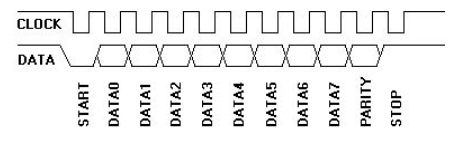
\includegraphics[scale=0.5]{ps2protocol.png}
   \caption{Comunicarea PS/2 dispozitiv-gazd\u{a}}
   \label{fig:ps2protocol}
  \end{center}
 \end{figure}

Datele transmise de la dispozitiv la gazd\u{a}  sunt citite pe frontul descendent al semnalului de tact. Frecven\cb{t}a acestui semnal trebuie sa fie \^{i}ntre 10 \cb{s}i 16.7 KHz. C\^{a}nd dispozitivul vrea sa transmit\u{a} date, mai \^{i}nt\^{a}i verific\u{a} dac\u{a} linia Clock e la nivelul logic high. Dac\u{a} nu, \^{i}nseamn\u{a} c\u{a} gazda inhib\u{a} comunicarea \cb{s}i dispozitivul va trebui s\u{a} re\cb{t}in\u{a} orice date de trimis p\^{a}n\u{a} c\^{a}nd gazda elibereaz\u{a} linia Clock. Dispozitivul trimite un bit pe linia Data c\^{a}nd Clock e high, iar gazda cite\cb{s}te c\^{a}nd Clock e low.}

\small{Procesorul tastaturii monitorizeaz\u{a} permanent matricea de taste. Dac\u{a} g\u{a}se\cb{s}te o tast\u{a} ce este ap\u{a}sat\u{a}, ridicat\u{a}, sau \cb{t}inut\u{a} jos, tastatura va trimite un pachet de informa\cb{t}ie numit\u{a} "scan code" c\u{a}tre calculator. Exist\u{a} dou\u{a} tipuri de scan code-uri: "make codes" \cb{s}i "break codes". Un make code este trimis atunci c\^{a}nd o tast\u{a} este ap\u{a}sat\u{a} sau \cb{t}inut\u{a} jos. Un break code este trimis atunci c\^{a}nd tasta este ridicat\u{a}. Fiecare tast\u{a} are propriul make code \cb{s}i break code. Mul\cb{t}imea de make code-uri si break code-uri a fiec\u{a}rei taste definesc un "scan code set". ~\cite{misc:ps2}}

\subsection{Filtre de imagini}

\subsubsection{Filtre de contrast} \label{filtrecontrast}
\small{Primul pas \^{i}n a calcula factorul de corec\cb{t}ie a contrastului este dat de formula: 
 \[  F =
\frac{259 * (C + 255) }{255 * (259 - C)}
\]

Valoarea C din formula denot\u{a} nivelul de contrast dorit. Urm\u{a}torul pas \^{i}l const\u{a} \^{i}n  ajustarea contrastului, aplic\^{a}nd urm\u{a}toarea formul\u{a} fiec\u{a}rei componente de culoare (R, G, B) din fiecare pixel:

 \[  
newRed = Truncate(F * (Red(color)   - 128) + 128)
\]
 \[  
newBlue = Truncate(F * (Blue(color)   - 128) + 128)
\]
 \[  
newGreen = Truncate(F * (Green(color)   - 128) + 128)
\]

De asemenea, trebuie s\u{a} trunchiem rezultatul astfel \^{i}nc\^{a}t acesta s\u{a} fie \^{i}ntre valorile acceptabile (0 \cb{s}i 255). Valoarea C poate fi \^{i}ntre -255 \cb{s}i 255. O valoare negativ\u{a} \^{i}nseamn\u{a} sc\u{a}derea nivelului de contrast, iar una pozitiv\u{a} cre\cb{s}terea acestuia. ~\cite{art:contrast}}

\subsubsection{Filtru grayscale}
Pentru a converti o imagine RGB \^{i}n grayscale, valoarea fiec\u{a}rui canal de culoare trebuie \^{i}nlocuit\u{a} cu media aritmetic\u{a} a canalelor. ~\cite{book:labpi}

\[C = \frac{R + G + B}{3}\]

\subsubsection{Filtru negativ}
Negativul unei imagini se poate ob\cb{t}ine calcul\^{a}nd complementul fiec\u{a}rui canal. ~\cite{book:labpi}

\[R' = 255 - R\]
\[G' = 255 - G\]
\[B' = 255 - B\]

\section{Proiectare \cb{s}i implementare}

 \begin{figure}
  \begin{center}
   \hspace*{-1.3in}
   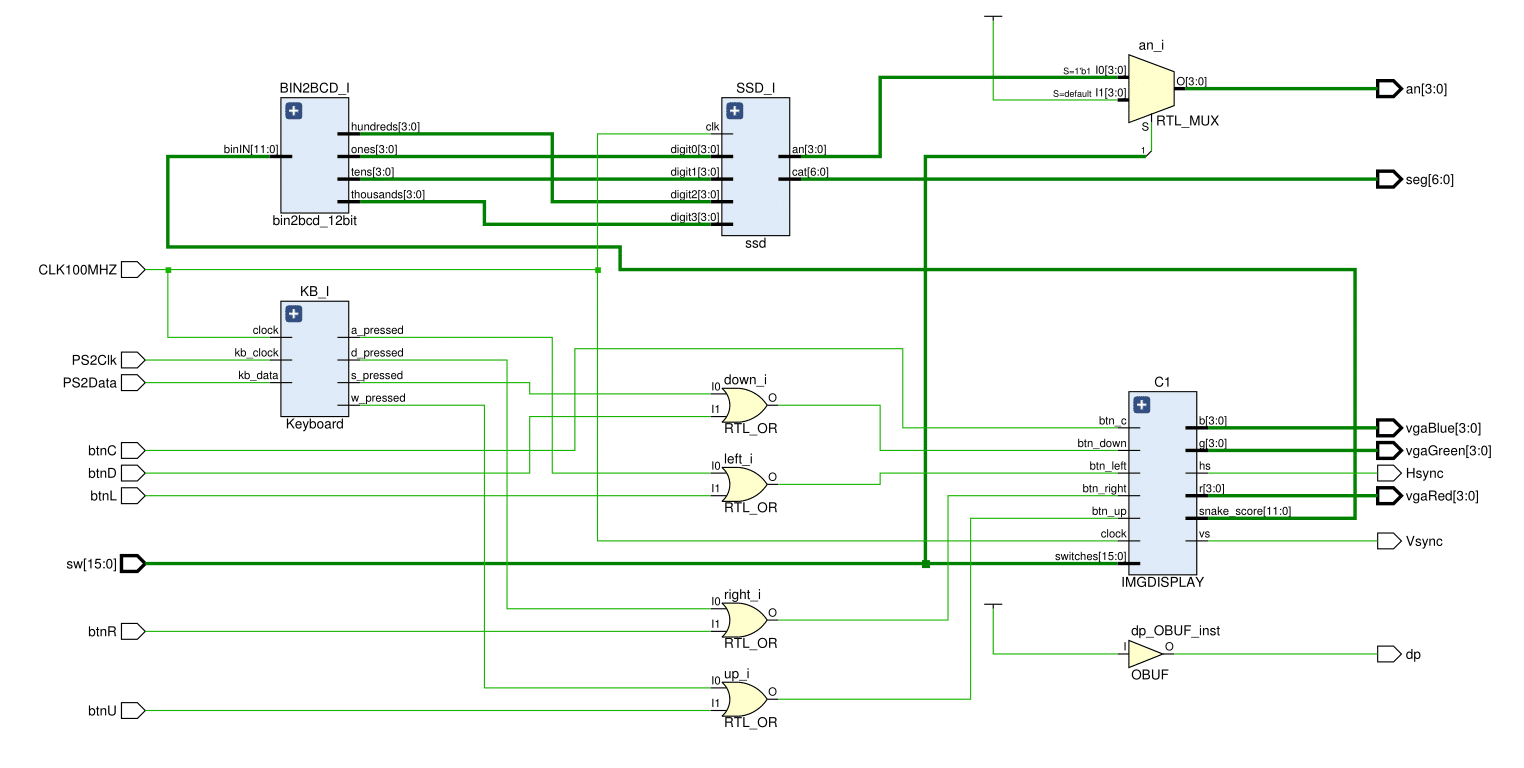
\includegraphics[scale=0.35]{schemabloc.png}
   \caption{Arhitectura general\u{a} a sistemului}
   \label{fig:schemabloc}
  \end{center}
 \end{figure}
\^{I}n Fig.\ref{fig:schemabloc} este prezentat\u{a} schema bloc a \^{i}ntregului sistem, \^{i}mpreun\u{a} cu porturile de I/O.
Porturile de intrare sunt urm\u{a}toarele:
\begin{itemize}
 \item CLK100MHZ - Semnalul de ceas al pl\u{a}cii de dezvoltare Basys 3. Acesta are o frecven\cb{t}\u{a} de 100 MHz;
 \item PS2Clk - Semnalul de ceas al tastaturii, corespunz\u{a}tor pinului Clock al conectorului PS/2 (Fig.\ref{fig:ps2pinout});
 \item PS2Data - Semnalul de date serial\u{a} a tastaturii, corespunz\u{a}tor pinului Data al conectorului PS/2 (Fig.\ref{fig:ps2pinout});
 \item sw - Comutatoarele pl\u{a}cii de dezvoltare. Acestea sunt utilizate pentru selecta imaginea afi\cb{s}at\u{a}, pentru a activa modulul Snake, precum \cb{s}i pentru a alege filtrele de imagini ce vor fi aplicate \^{i}nainte de afi\cb{s}are;
 \item btnC - Butonul central al pl\u{a}cii de dezvoltare. Este utilizat pentru a reseta modulul Snake;
 \item btnU, btnD, btnL, btnR - Butoanele de sus, jos, st\^{a}nga, respectiv dreapta ale pl\u{a}cii de dezvoltare. Sunt utilizate pentru a controla directia \cb{s}arpelui \^{i}n modulul Snake.
\end{itemize}

Porturile de ie\cb{s}ire sunt urm\u{a}toarele:
\begin{itemize}
 \item HSync - Semnalul de sincronizare orizontal\u{a} al conectorului VGA. (Fig.\ref{fig:vgaconnector});
 \item VSync - Semnalul de sincronizare vertical\u{a} al conectorului VGA. (Fig.\ref{fig:vgaconnector});
 \item vgaRed - Componenta ro\cb{s}ie a pixelului trimis la monitor prin conectorul VGA;
 \item vgaGreen - Componenta verde a pixelului trimis la monitor prin conectorul VGA;
 \item vgaBlue - Componenta albastr\u{a} a pixelului trimis la monitor prin conectorul VGA;
 \item an - Anozii afi\cb{s}oarelor cu 7 segmente ale pl\u{a}cii de dezvoltare;
 \item seg - Catozii afi\cb{s}oarelor cu 7 segmente ale pl\u{a}cii de dezvoltare;
 \item dp - Catodul corespunz\u{a}tor punctului afi\cb{s}oarelor cu 7 segmente ale pl\u{a}cii de dezvoltare. Acesta este mereu '1' logic (punctul este stins).
\end{itemize}

Afi\cb{s}oarele cu 7 segmente sunt folosite pentru a afi\cb{s}a scorul juc\u{a}torului \^{i}n Snake. Afi\cb{s}oarele sunt dezactivate atunci c\^{a}nd modulul Snake este inactiv.

Componenta ``IMGDISPLAY'' controleaz\u{a} afi\cb{s}area imaginilor pe display. Aceasta con\cb{t}ine controller-ul interfe\cb{t}ei VGA, memoria cu imaginile ce pot fi afi\cb{s}ate, precum \cb{s}i modulul Snake.

Componenta ``Keyboard'' cite\cb{s}te serial datele de la conectorul PS/2 \cb{s}i detecteaz\u{a} ap\u{a}sarea tastelor W, A, S, D - utilizate pentru a controla \cb{s}arpele.

Componenta ``bin2bcd\_12bit'' realizeaz\u{a} conversia unui num\u{a}r unsigned pe 12 bi\cb{t}i la un num\u{a}r \^{i}n reprezentarea BCD.

Componenta ``ssd'' se ocup\u{a} de afi\cb{s}area numarului BCD pe display-ul cu 7 segmente.

\subsection{Afi\cb{s}area imaginilor}

Pentru afi\cb{s}area imaginilor, modulul ``IMGDISPLAY'' con\cb{t}ine componenta ``Vga\_Controller'', care prime\cb{s}te semnalul PixelClock (semnal de tact cu frecven\cb{t}a de 25 MHz - la fiecare puls al acestuia se va trimite informa\cb{t}ia de culoare a unui anumit pixel) \cb{s}i produce urm\u{a}toarele semnale:
\begin{itemize}
 \item HS - Sincronizare orizontal\u{a}, acest semnal comunic\u{a} dizpozitivului de afi\cb{s}are faptul c\u{a} am terminat de afi\cb{s}at un r\^{a}nd \cb{s}i dorim trecerea fasciculului de electroni la \^{i}nceputul r\^{a}ndului urm\u{a}tor;
 \item VS - Sincronizare vertical\u{a}, acest semnal comunic\u{a} dizpozitivului de afi\cb{s}are faptul c\u{a} am terminat de afi\cb{s}at \^{i}ntregul cadru \cb{s}i dorim trecerea fasciculului de electroni \^{i}n col\cb{t}ul st\^{a}nga sus al ecranului, pentru afi\cb{s}area unui cadru nou;
 \item H - Vector de zece bi\cb{t}i, reprezint\u{a} pozi\cb{t}ia orizontal\u{a} (coordonata X), a fasciculului de electroni, respectiv a pixelului curent;
 \item V - Vector de zece bi\cb{t}i, reprezint\u{a} pozi\cb{t}ia vertical\u{a} (coordonata Y), a fasciculului de electroni, respectiv a pixelului curent;
 \item Blank - Acest semnal este activ dac\u{a} valorile semnalelor H \cb{s}i V nu reprezint\u{a} pozi\cb{t}ii de pixeli valide. \^{I}ntre trecerile dintre linii sau cadre, este nevoie de timp suplimentar pentru sincronizare, \^{i}n care informa\cb{t}ia de culoare nu va fi transmis\u{a}, ci se va trimite culoarea neagr\u{a} / blank (valorile R, G \cb{s}i B vor fi zero), deoarece atunci monitorul va fi nevoit sa \^{i}\cb{s}i calibreze culorile.
\end{itemize}

Semnalele H \cb{s}i V sunt folosite pentru a forma o adres\u{a} ce va indexa culoarea dintr-o memorie ROM ce con\cb{t}ine o imagine, precum \cb{s}i pentru a determina dac\u{a} pixelul curent con\cb{t}ine un obiect \^{i}n modulul Snake.

De\cb{s}i acest controller este capabil de a afi\cb{s}a imagini la o rezolu\cb{t}ie de 640x480, datorit\u{a} resurselor hardware (capacitatea de memorie a pl\u{a}cii de dezvoltare FPGA) limitate, imaginile afi\cb{s}ate sunt reduse la 160x120 (de 4 ori \^{i}n fiecare dimensiune). \^{I}n acest demers, numerele reprezentate de semnalele H \cb{s}i V au fost \cb{i}mp\u{a}r\cb{t}ite cu 4. Astfel, c\^{a}te 16 combina\cb{t}ii ale valorilor semnalelor H \cb{s}i V vor adresa aceea\cb{s}i loca\cb{t}ie de memorie. Pentru modulul Snake, se folosesc semnale H \cb{s}i V \^{i}mp\u{a}r\cb{t}ite la 8, deci rezolu\cb{t}ia jocului va fi 80x60.

Acest controller VGA a fost implementat utiliz\^{a}nd dou\u{a} num\u{a}r\u{a}toare ca module principale. Primul num\u{a}r\u{a}tor va num\u{a}ra pozi\cb{t}ia orizontal\u{a} a pixelului. Dup\u{a} ce a terminat secven\cb{t}a de num\u{a}rare, se va reseta la zero iar al doilea num\u{a}r\u{a}tor va num\u{a}ra o singur\u{a} dat\u{a}. \^{I}n Fig.\ref{fig:vgactl} este prezentat\u{a} schema bloc a acestei implement\u{a}ri. Semnalul Blank inversat a fost aplicat la intrarea multiplexorului pentru a decide dac\u{a} se va transmite informa\cb{t}ia de culoare sau valoarea zero.

\begin{figure}
  \begin{center}
   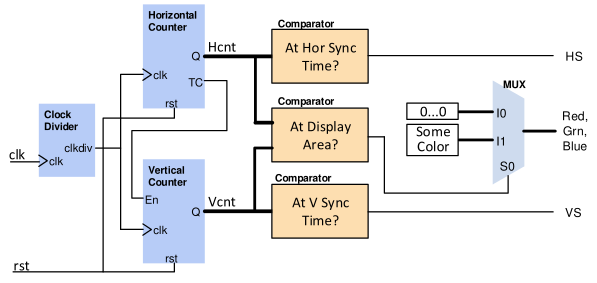
\includegraphics[scale=0.5]{VGA_BlockDiagram.png}
   \caption{Implementarea controller-ului VGA}
   \label{fig:vgactl}
  \end{center}
 \end{figure}
 
 \^{I}n Fig.\ref{fig:vgatiming} este prezentat\u{a} diagrama de timp a semnalelor VGA. Din aceasta putem deduce urm\u{a}toarele intervale de timp:
 \[t_{hs}, t_{hpb}, t_{hfp}, t_{haddr}, t_{hbd}, t_{vs}, t_{vbp}, t_{vfp}, t_{vaddr}, t_{vbd}\]
 Aceste intervale sunt descrise \^{i}n tabelul \ref{table:vgatimes}, \^{i}mpreun\u{a} cu duratele lor.
    Vom afi\cb{s}a informa\cb{t}ie video doar atunci c\^{a}nd num\u{a}r\u{a}torul orizontal se afl\u{a} \^{i}n $t_{\text{haddr}}$ (are valoarea mai mic\u{a} dec\^{a}t $H_{\text{max_{addr}}}$) iar num\u{a}r\u{a}torul vertical se afl\u{a} \^{i}n $t_{\text{vaddr}}$ (are valoarea mai mic\u{a} dec\^{a}t $V_{\text{max_{addr}}}$).
 \^{I}n toate celelalte intervale de timp, informa\cb{t}ia de culoare va fi ``blanked''. Semnalele HS \cb{s}i VS vor fi active doar \^{i}n timpii $t_{\text{hs}}$, respectiv $t_{\text{vs}}$.
 
 Cu ajutorul specifica\cb{t}iei timpilor din tabelul \ref{table:vgatimes}, putem calcula valorile maxime ale num\u{a}r\u{a}toarelor:
 
 \[
  H_{max} = \frac{t_{hs} + t_{hbp} + t_{hfp} + t_{haddr} + t_{hbd}}{t_{clk}} = 800
 \]
 
 \[
  V_{max} = \frac{t_{vs} + t_{vbp} + t_{vfp} + t_{vaddr} + t_{vbd}}{t_{hs} + t_{hbp} + t_{hfp} + t_{haddr} + t_{hbd}} = 525
 \]
 
 \[
  H_{max_{addr}} = \frac{t_{haddr}}{t_{clk}} = 640
 \]
 
  \[
  V_{max_{addr}} = \frac{t_{vaddr}}{t_{hs} + t_{hbp} + t_{hfp} + t_{haddr} + t_{hbd}} = 480
 \]

 \begin{figure}
  \begin{center}
   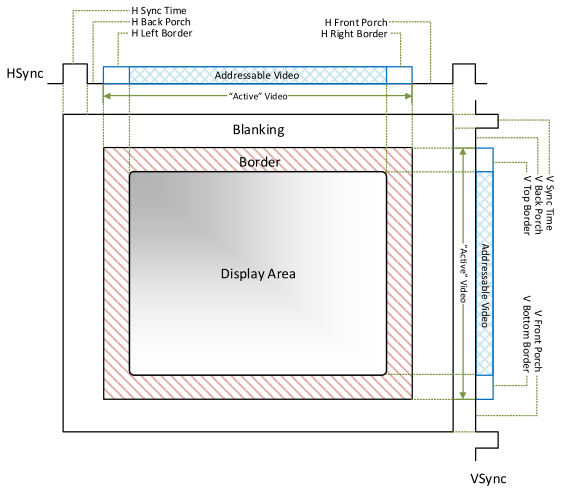
\includegraphics[scale=0.5]{VESA_TimingDiagram.png}
   \caption{Diagrama de timp pentru sincronizarea semnalelor VGA}
   \label{fig:vgatiming}
  \end{center}
 \end{figure}
 
 \begin{table}
\begin{center}
 \begin{tabular}{ || c | c | c | c || }
  \hline \hline
  \textbf{Descriere} & \textbf{Nota\cb{t}ie} & \textbf{Timp} & \textbf{Timp/Frecven\cb{t}a} \\
  \hline
  Pixel Clock & t_{clk} & 39.7 ns & 25.175MHz \\
  H Sync Time & t_{hs} & 3.813 \mu s & 96 Pixeli \\
  H Back Porch & t_{hbp} & 1.907 \mu s & 48 Pixeli \\
  H Front Porch & t_{hfp} & 0.636 \mu s & 16 Pixeli \\
  H Addr Video Time & t_{haddr} & 25.422 \mu s & 640 Pixeli \\
  H L/R Border & t_{hbd} & 0 \mu s & 0 Pixeli \\
  V Sync Time & t_{vs} & 0.064 ms & 2 Linii \\
  V Back Porch & t_{vbp} & 1.048 ms & 33 Linii \\
  V Front Porch & t_{vfp} & 0.318 ms & 10 Linii \\
  V Addr Video Time & t_{vaddr} & 15.253 ms & 480 Linii \\
  V T/B Border & t_{vbd} & 0 ms & 0 Linii \\
  \hline \hline
 \end{tabular}
\end{center}
 \caption{Specifica\cb{t}ia timpilor pentru controller-ul VGA}
 \label{table:vgatimes}
\end{table}

Pentru a calcula adresa pentru indexarea pixelului dintr-o memorie cu o imagine, se \^{i}nmul\cb{t}e\cb{s}te V cu 160 (lungimea imaginii), iar apoi se adun\u{a} cu H. Trebuie men\cb{t}ionat faptul c\u{a} se folosesc semnalele H \cb{s}i V \^{i}mp\u{a}r\cb{t}ite la 4.

\subsection{Filtre de imagini} \label{impartirejmk}

La implementarea filtrului de contract sc\u{a}zut, \^{i}n formulele din sec\cb{t}iunea \ref{filtrecontrast}, a fost ales:

\[F = \frac{1}{4}\]

astfel \^{i}ncat s\u{a} se poat\u{a} realiza \^{i}mp\u{a}r\cb{t}irea c\^{a}t mai rapid, cu o deplasarea la dreapta cu doi bi\cb{t}i.
Similar, pentru filtrul de contrast ridicat, pentru a se putea realiza u\cb{s}or \^{i}nmul\cb{t}irea cu o deplasare la st\^{a}nga cu doi bi\cb{t}i, s-a ales:

\[F = 4\]

Pentru a realiza conversia imaginii \^{i}n grayscale, este nevoie de a executa opera\cb{t}ia de \^{i}mp\u{a}r\cb{t}ire la 3, pentru ob\cb{t}inerea medii aritmetice a valorilor cananelor fiec\u{a}rui pixel.
Aceast\u{a} opera\cb{t}ie trebuie f\u{a}cut\u{a} rapid, astfel \^{i}nc\^{a}t ar trebui s\u{a} dureze mai pu\cb{t}in de 40 ns (un pixel trebuie trimis spre afi\cb{s}are la fiecare 25 MHz).
Ne putem folosi de faptul c\u{a} mereu \^{i}mp\u{a}r\cb{t}itorul opera\cb{t}iei este 3, \cb{s}i astfel am proiectat un circuit specializat ce realizeaza doar opera\cb{t}ii de \^{i}mp\u{a}r\cb{t}ire a numerelor la 3.
Circuitul ob\cb{t}inut este unul iterativ, component\u{a} necesar\u{a} fiind un \^{i}mp\u{a}r\cb{t}itor de numere pe 4 bi\cb{t}i la 3. Acesta a fost implementat ca un lookup table, lu\^{a}nd \^{i}n considerare num\u{a}rul mic de combina\cb{t}ii ale intr\u{a}rilor - 16.
Fiecare component\u{a} va calcua un c\u{a}t par\cb{t}ial \cb{s}, folosind restul par\cb{t}ial de la opera\cb{t}ia precedent\u{a} \^{i}mpreun\u{a} cu 2 bi\cb{t}i din de\^{i}mp\u{a}r\cb{t}it.
La intrarea fiec\u{a}rei componente vor fi aplica\cb{t}i c\^{a}te 2 bi\cb{t}i ai de\^{i}mp\u{a}r\cb{t}itului concatena\cb{t}i la st\^{a}nga cu restul par\cb{t}ial de la componenta anterioar\u{a}. Pentru prima component\u{a}, consider\u{a}m restul anterior ca fiind zero.

 \begin{figure}
  \begin{center}
   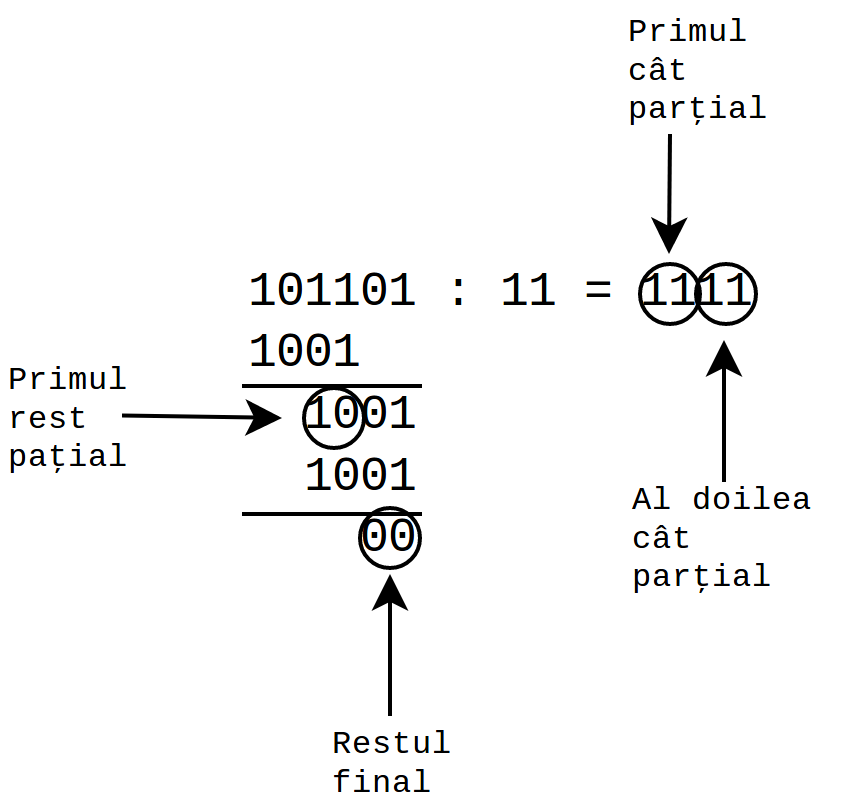
\includegraphics[scale=0.25]{impartire.png}
   \caption{Exemplificarea algoritmului de \^{i}mp\u{a}r\cb{t}ire la 3}
   \label{fig:division3}
  \end{center}
 \end{figure}

\subsection{Modulul Snake} \label{sneic}

Jocul ruleaz\u{a} la rezolu\cb{t}ia de 80x60 pixeli. \^{I}n jocul Snake exist\u{a} dou\u{a} obiecte: \cb{s}arpele \cb{s}i m\^{a}ncarea.
M\^{a}ncarea este reprezentat\u{a} cu un pixel. Aceasta \^{i}\cb{s}i va schimba pozi\cb{t}ia de fiecare dat\u{a} c\^{a}nd intr\u{a} \^{i}n contact cu \cb{s}arpele.
Aceast\u{a} pozi\cb{t}ie este memorat\u{a} \^{i}ntr-un registru de date.
\cb{S}arpele este alc\u{a}tuit dintr-un num\u{a}r variabil de segmente. Acest num\u{a}r cre\cb{s}te de fiecare dat\u{a} c\^{a}nd capul (primul segment) intr\u{a} \^{i}n contact cu m\^{a}ncarea.
C\^{a}nd jocul \^{i}ncepe, \cb{s}arpele are patru segmente. Coordonatele segmentelor sunt memorate \^{i}ntr-o serie de regi\cb{s}tri care se comport\u{a} ca o stiv\u{a}.
Alt registru este folosit pentru a memora direc\cb{t}ia \cb{s}arpelui. Exist\u{a} patru direc\cb{t}ii posibile (sus, jos, st\u{a}nga, dreapta), astfel 2 bi\cb{t}i fiind suficien\cb{t}i.
Valoarea din acest registru se va schimba la primirea comenzilor (de la tastatur\u{a}, butoanele de pe placa de dezvolate).
\^{I}ntr-un ultim registru este \cb{t}inut scorul ob\cb{t}inut. Ini\cb{t}ial zero, acesta cre\cb{s}te la fiecare coliziune a \cb{s}arpelui cu m\^{a}ncarea. Aceast\u{a} valoare va fi afi\cb{s}at\u{a} pe afi\cb{s}oarele cu 7 segmente.

\^{I}n fiecare registru din stiv\u{a} va fi re\cb{t}inut \cb{s}i un bit V, care determin\u{a} dac\u{a} segmentul cu acea pozi\cb{t}ie face parte din \cb{s}arpe. Avem nevoie de un astfel de bit deoarece num\u{a}rul de segmente este variabil, \^{i}n timp ce num\u{a}rul de registre este fix. \^{I}n fiecare cadru este calculat\u{a} pozi\cb{t}ia urm\u{a}toare a capului \cb{s}arpelui, \^{i}n func\cb{t}ie de direc\cb{t}ie.
La momentul mi\cb{s}c\u{a}rii, pe stiv\u{a} este dat push la noua pozi\cb{t}ie. Astfel, capul \cb{s}arpelui fiind acum la pozi\cb{t}ia nou calculat\u{a}, registrele urm\u{a}toare iau succesiv valorile registrelor anterioare. Bitul V al valorii nou introduse va fi 1.
Totu\cb{s}i, valorile bi\cb{t}ilor V \^{i}\cb{s}i vor p\u{a}stra valoarea, deoarece nu vrem ca num\u{a}rul de segmente s\u{a} creasc\u{a}.
La momentul coliziunii cu m\^{a}ncarea, deoarece dorim \cb{s}i cre\cb{s}terea num\u{a}rului de segmente, vom deplasa inclusiv \cb{s}i valorile bi\cb{t}ilor V.
De asemenea, este folosit un generator de numere aleatoare pentru a genera o nou\u{a} pozi\cb{t}ie pentru m\^{a}ncare \cb{s}i va fi incrementat scorul.

Generatorul de numere aleatoare a fost implementat cu algoritmul Xorshift.
Conversia scorului \^{i}ntr-un num\u{a}r BCD, pentru  a fi afi\cb{s}at, este realizat\u{a} cu algoritmul Double dabble.

Dou\u{a} intr\u{a}ri ale acestui modul, X \cb{s}i Y, coordonatele pixelului curent ale controller-ului VGA, \^{i}mp\u{a}r\cb{t}ite la 8, sunt comparate cu fiecare valoare din registrele stiv\u{a} \cb{s}i cu valoarea din registrul pentru m\^{a}ncare.
Dac\u{a} exist\u{a} cel pu\cb{t}in o egalitate \^{i}ntre coordonatele de la intrare \cb{s}i cele men\cb{t}ionate anterior, iar, in cazul egalit\u{a}\cb{t}ii cu o valoare dintr-un registru stiv\u{a}, bitul V este 1, atunci ie\cb{s}irea ``Pixel On'' va fi 1, iar \^{i}n caz contrar 0.
Aceast\u{a} ie\cb{s}ire va determina dac\u{a} pixelul care urmeaz\u{a} s\u{a} fie desenat pe ecran con\cb{t}ine un obiect din joc (\cb{s}arpe sau m\^{a}ncare).
Culoarea alb\u{a} reprezint\u{a} prezen\cb{t}a unui obiect, \^{i}n timp ce culoarea neagr\u{a} absen\cb{t}a acestuia. Aceast\u{a} culoare va trece apoi prin filtrele de imagini.

Stiva a fost proiectat\u{a} ca un modul generic, exist\^{a}nd posibilitatea schimb\u{a}rii num\u{a}rului de regi\cb{s}tri prin modificarea unei constante.
Pentru implementarea curent\u{a}, aceast\u{a} constant\u{a} a fost setat\u{a} pe 256. Acest num\u{a}r determin\u{a} num\u{a}rul maxim de segmente pe care \^{i}l poate avea \cb{s}arpele.
Deoarece acest num\u{a}r determin\u{a} \cb{s}i num\u{a}rul de compara\cb{t}ii cu coordonatele de la intrare, acesta nu trebuie s\u{a} fie prea mare, pentru ca timpul de calcul s\u{a} se \^{i}ncadreze, \^{i}mpreun\u{a} cu celelalte calcule \cb{s}i \^{i}nt\^{a}rzieri, \^{i}n perioada semnalului ``Pixel Clock''.

Un num\u{a}r suplimentar de comparatoare este necesar pentru a verifica coliziunea capului \cb{s}arpelui cu restul corpului s\u{a}u. Dac\u{a} exist\u{a} o egalitate \^{i}ntre coordonatele capului \cb{s}i una din coordonatele celorlalte segmente, iar bitul V al segmentului cu a c\u{a}rui coordonate sunt egale este 1, atunci exist\u{a} coliziune.
\^{I}n caz c\u{a} exist\u{a} coliziune, jocul se va termina. \^{I}n acel moment, scorul va fi resetat la zero, pozi\cb{t}ia \cb{s}arpelui va fi resetat\u{a} la coordonatele ini\cb{t}iale, num\u{a}rul de segmente la 4, iar m\^{a}ncarea va primi o nou\u{a} pozi\cb{t}ie aleatoare.

 \begin{figure}
  \begin{center}
   
\includegraphics[scale=0.2]{snek.png}
   \caption{\cb{S}arpe}
   \label{fig:snake}
  \end{center}
 \end{figure}

\subsection{Citirea tastelor}

Controller-ul PS/2 a fost realizat cu ajutorul unui registru de deplasare pe 11 bi\cb{t}i. Pinul Clock al conectorului PS/2 este conectat la intrarea Clock al registrului, iar pinul Data la intrarea serial\u{a} a acestuia.
Un num\u{a}r\u{a}tor num\u{a}r\u{a} bi\cb{t}ii recep\cb{t}iona\cb{t}i. Atunci c\^{a}nd a num\u{a}rat 11 bi\cb{t}i, se verific\u{a} dac\u{a} bitul de start, bitul de stop \cb{s}i bitul de paritate corespund specifica\cb{t}iei PS/2.
Dac\u{a} acesta este cazul, este interpretat scan code-ul \cb{s}i se verific\u{a} dac\u{a} acesta corespunde uneia dintre tastele W, A, S, D. Starea acestor butoane (dac\u{a} este ap\u{a}sat sau nu) este memorat\u{a} \^{i}ntr-un set de 4 bistabile.
Dac\u{a} scan code-ul este un make code, atunci starea bistabilului va deveni 1, iar dac\u{a} este un break code, va deveni 0.
Starea acestor taste, va fi folosit\u{a} mai departe \^{i}n modulul Snake.

\section{Rezultate experimentale}

\subsection{Instrumente utilizate}

Proiectul a fost implementat \^{i}n limbajul de descriere hardware VHDL, \^{i}n mediul de dezvoltare Xilinx Vivado 2017.4, pentru placa de dezvoltare Xilinx Basys 3 Artix-7 FPGA.
Dezvoltarea proiectului a avut loc pe un laptop Asus F550J, cu sistemul de operare Microsoft Windows 10 64-bit. Alte instrumente utilizate la dezvoltare sunt un monitor LG 24MP68VQ-P \cb{s}i o tastatur\u{a} Cooler Master STORM QuickFire XT MX Brown.

\subsection{Circuitul implementat}

\^{I}n tabelul \ref{table:implementation} sunt prezentate informa\cb{t}iile din rapoartele de implementare oferite de mediul de dezvoltare Vivado.

\begin{table}
\begin{center}
 \begin{tabular}{ | c | c | }
  \hline
  Utilizare LUT & 5377 \\
  \hline
  Utilizare FF & 3912 \\
  \hline
  Utilizare BRAM & 24 \\
  \hline
  Utilizare IO & 58 \\
  \hline
  Utilizare BUFG & 1 \\
  \hline
  Frecven\cb{t}a maxim\u{a} & 129.6 MHz \\
  \hline
  Puterea total\u{a} & 0.128 W \\
  \hline
  Temperatura & 25.6 $^\circ$C \\
  \hline
 \end{tabular}
\end{center}
 \caption{Informa\cb{t}ii din rapoartele de implementare}
 \label{table:implementation}
\end{table}

Calea critic\u{a} a \^{i}ntregului circuit este reprezentat\u{a} de comparatoarele din modulul Snake (sec\cb{t}iunea \ref{sneic}). Dac\u{a} cre\cb{s}tem num\u{a}rul registrelor din stiv\u{a} \cb{s}i, implicit, num\u{a}rul comparatoarelor, vom observa o sc\u{a}dere a frecven\cb{t}ei maxime.
Totu\cb{s}i, valoarea ob\cb{t}inut\u{a} p\^{a}n\u{a} acum este destul de departe de valoarea minim\u{a} de care avem nevoie (25 MHz), deci s-ar putea experimenta cu un num\u{a}r mai mare de registre.

\subsection{Testare}

Pentru testarea sistemului, a fost utilizat simulatorul Vivado. A fost scris un banc de test pentru \^{i}mp\u{a}r\cb{t}itorul la 3, \^{i}n care a fost aplicat un num\u{a}r de 64 de vectori de test. Testele au fost trecute cu succes, dup\u{a} cum se poate observa \^{i}n Fig. \ref{fig:sim}.

 \begin{figure}
  \begin{center}
   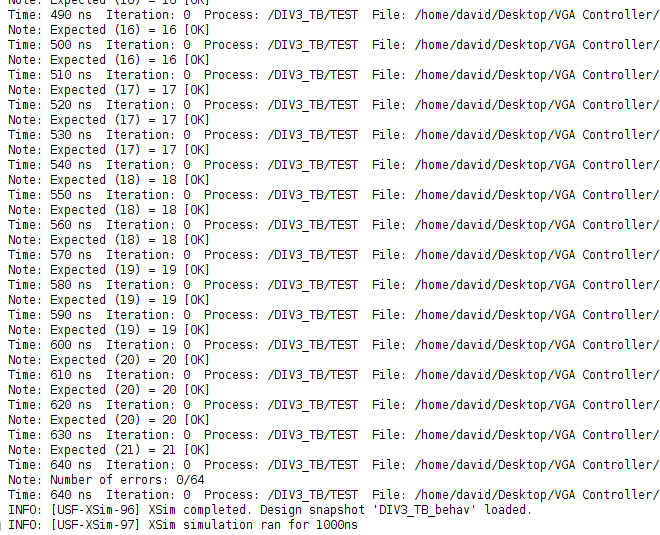
\includegraphics[scale=0.5]{sim.png}
   \caption{Rezultatele simul\u{a}rii \^{i}mp\u{a}r\cb{t}itorului la 3}
   \label{fig:sim}
  \end{center}
 \end{figure}

\section{Concluzii}

Problema rezolvat\u{a} a fost aceea a intefa\cb{t}\u{a}rii conectorului VGA, \^{i}n vederea afi\cb{s}\u{a}rii imaginilor pe un display cu conectivitate VGA.
Obiectivul ini\cb{t}ial a fost acela a afi\cb{s}\u{a}rii unei imagini statice color pe un display.
Scrierea imaginii \^{i}ntr-o memorie ROM ar fi fost o sarcin\u{a} lung\u{a} \cb{s}i obisitoare. Pentru a rezolva aceast\u{a} problem\u{a}, a fost dezvoltat\u{a} o aplica\cb{t}ie \^{i}n C++ cu libr\u{a}ria OpenCV, care prime\cb{t}e o imagine la intrare \cb{s}i genereaz\u{a} un fi\cb{s}ier surs\u{a} VHDL cu memoria ROM ce con\cb{t}ine culorile pixelilor imaginii.
Pentru a putea stoca o imagine la rezolu\cb{t}ia nativ\u{a} (640x480), Block RAM-ul pl\u{a}cii de dezvoltare nu ar fi fost suficient, astfel imaginea a fost redus\u{a} ca dimensiune de c\u{a}tre aplica\cb{t}ia men\cb{t}ionat\u{a} anterior \cb{s}i s-a efectuat o opera\cb{t}ie de scalare pe coordonatele pixelilor.
Un ultim pas de procesare a imaginii \^{i}nainte de scrierea memoriei a fost reducerea gamei de valori a fiec\u{a}rui canal de culoare de la 0-255 la 0-15, printr-o deplasare la dreapta cu 4 bi\cb{t}i, deoarece rezolu\cb{t}ia convertorului digital-analog al pl\u{a}cii de dezvoltare - ce este utilizat pentru a converti canalele de culoare \^{i}n analog pentru a le putea transmite prin pinii vgaRed, vgaGreen \cb{s}i vgaBlue c\u{a}tre display - este de 4 bi\cb{t}i. 
Acest obiectiv fiind \^{i}ndeplinit \^{i}ntr-un timp relativ scurt \cb{s}i, neexist\^{a}nd constr\^{a}ngeri de timp, au mai fost stabilite alte trei obiective:
\begin{itemize}
 \item Aplicarea unor filtre de imagini prin modificarea valorilor cananelor de culoare \^{i}n timpul execu\cb{t}iei.
 A fost necesar ca filtrele s\u{a} fie componente combina\cb{t}ionale mici care vor executa calcule rapid, pentru a nu introduce \^{i}nt\^{a}rzieri semnificative.
 O provocare a fost filtrul grayscale, care necesit\u{a} o \^{i}mp\u{a}r\cb{t}ire la 3. \^{I}n sec\cb{t}iunea \ref{impartirejmk} este prezentat algoritmul de \^{i}mp\u{a}r\cb{t}ire.
 \item Afi\cb{s}area de imagini dinamice, interactive, care r\u{a}spund la stimulii utilizatorului. Acest obiectiv s-a concretizat prin dezvoltarea unui joc 2D simplu, mai exact o implementare a jocului Snake. Acest gen de joc a avut debutul \^{i}n anul 1976, pe hardware-ul de jocuri arcade Blockade ~\cite{wiki:snake}. Astfel, datorit\u{a} trivialit\u{a}\cb{t}ii de implementare \cb{s}i a resurselor hardware necesare reduse, a fost aleas\u{a} aceast\u{a} aplica\cb{t}ie.
 O dificultate a reprezentat-o posibilitatea ca \cb{s}arpele s\u{a} se poat\u{a} \^{i}ntoarce direct, \^{i}n direc\cb{t}ia opus\u{a}, la 180$^\circ$. O astfel de mutare avea drept consecin\cb{t}\u{a} imediat\u{a} sf\^{a}r\cb{s}itul jocului. A trebuit implementat\u{a} o restric\cb{t}ionare a mi\cb{s}c\u{a}rilor posibile, prin ad\u{a}ugarea de logic\u{a} suplimentar\u{a} la intrarea Write Enable a registrului de direc\cb{t}ie.
 Datorit\u{a} num\u{a}rului mare de registre \cb{s}i por\cb{t}i logice, a fost aleas\u{a} o implementare de tip for...generate, pentru a reduce dimensiunea codului, pentru a cre\cb{s}te simplitatea \cb{s}i lizibilitatea, dar \cb{s}i pentru a putea aduce modific\u{a}ri cu u\cb{s}urin\cb{t}\u{a}.
 Pe parcursul dezvolt\u{a}rii, a fost modificat \^{i}n mod repetat num\u{a}rul de registre din stiva \cb{s}arpelui, test\^{a}nd de fiecare dat\u{a} func\cb{t}ionalitatea corect\u{a} a modulului.
 \item Preluarea de input de la o tastatur\u{a} PS/2 pentru a interc\cb{t}iunea cu utilizatorul. Au existat anumite dificult\u{a}\cb{t}i legate de sincronizarea semnalelor, ce au fost rezolvate prin experimentarea cu diferite \^{i}nt\^{a}rzieri introduse artificial.
 \end{itemize}


\subsection{Dezvolt\u{a}ri viitoare}

O posibil\u{a} dezvoltare ulterioar\u{a} ar putea fi ad\u{a}ugarea unui microprocesor cu intruc\cb{t}iuni speciale de manipulare a unei memorii video (framebuffer).
Controller-ul VGA va afi\cb{s}a pe display informa\cb{t}iile din acest framebuffer. Mai multe jocuri ar putea fi scrise \^{i}n cod ma\cb{s}in\u{a} pentru acest microprocesor (Pong, Asteroids, Tetris, Breakout). Astfel, acest proiect ar deveni o platform\u{a} de jocuri de tipul jocurilor arcade din anii 1970-1980.

Alte posibile dezvolt\u{a}ri, dar care ar putea necesita o plac\u{a} de dezvoltare cu mai mult\u{a} putere de procesare:
\begin{itemize}
 \item Exemplificare de randare 3D cu un ray tracer;
 \item Video streaming de pe re\cb{t}ea. Este necesar un port de ethernet \cb{s}i ie\cb{s}ire audio;
 \item Afi\cb{s}area de date despre stock market sau pia\cb{t}a criptomonedelor sub form\u{a} de grafice \cb{s}i tabele. Preluarea datelor se va face de la un server;
 \item Display interactiv pentru a afi\cb{s}a informa\cb{t}ii despre loca\cb{t}ie sau \^{i}mprejurimi \^{i}ntr-un loc public, cum ar fi un mall, o gr\u{a}din\u{a} zoo, un muzeu, sau alte locuri vizitate de turi\cb{s}ti;
 \item Vizualizator sub form\u{a} de unde luminoase pentru muzic\u{a}.
\end{itemize}


\newpage

\bibliography{ssc.bib}{}
\bibliographystyle{plain}


\end{document}